% MSRI - SGS Sparsity week 1, Monday, 2 lectures, 60 minutes each

\documentclass{beamer}

\usepackage{amsmath,amssymb,amsthm,mathrsfs,amscd}
\usepackage{datetime}
\usepackage{csquotes}
\usepackage{hyperref}
\usepackage{graphicx}
\usepackage{tikz,tikz-cd}
\usetikzlibrary{arrows,shapes}

\usetheme{Metropolis}
\metroset{block=fill}



\newcounter{maincounter}
\newcounter{excounter}

\newtheorem{conjecture}{Conjecture}
% \setbeamercolor{block body}{bg=mDarkTeal!15}
% \setbeamercolor{block title}{bg=mDarkTeal,fg=black!2}


\newcounter{maincounter}
\newcounter{excounter}
\numberwithin{maincounter}{chapter}
\numberwithin{equation}{chapter}
\numberwithin{excounter}{chapter}
\renewcommand{\theexcounter}{\thechapter.\Alph{excounter}}
\newtheorem{lemma}[maincounter]{Lemma}
\newtheorem{proposition}[maincounter]{Proposition}
\newtheorem{corollary}[maincounter]{Corollary}
\newtheorem{remark}[maincounter]{Remark}
\newtheorem{theorem}[maincounter]{Theorem}
\newtheorem{exercise}[excounter]{Exercise}
\newtheorem{example}[maincounter]{Example}

\newtheorem*{crucial}{Crucial Observation}

\newtheorem{conjecture}[maincounter]{Conjecture}
\newtheorem{definition}[maincounter]{Definition}

\def\AA{\mathbb{A}}
\def\BB{\mathbb{B}}
\def\EE{\mathbb{E}}
\def\HH{\mathbb{H}}
\def\DD{\mathbb{D}}
\def\NN{\mathbb{N}}
\def\RR{\mathbb{R}}
\def\TT{\mathbb{T}}
\def\CC{\mathbb{C}}
\def\ZZ{\mathbb{Z}}
\def\PP{\mathbb{P}}
\def\QQ{\mathbb{Q}}
\def\FF{\mathbb{F}}
\def\GG{\mathbb{G}}
\def\LL{\mathbb{L}}
\def\MM{\mathbb{M}}
\def\SS{\mathbb{S}}
\def\UU{\mathbb{U}}
\def\XX{\mathbb{X}}


%%% Philipp's macros

\newcommand{\dom}[1]{{\mathrm {dom}}({#1})}
\newcommand{\sman}[1]{{#1}^{\mathrm{sm,an}}}
\newcommand{\ansm}[1]{{#1}^{\mathrm{an,sm}}}
\newcommand{\sm}[1]{{#1}^{\mathrm{sm}}}
\newcommand{\anE}{\mathrm{an}}
\newcommand{\an}[1]{{#1}^{\anE}}
\newcommand{\stab}[1]{{\mathrm{Stab}(#1)}}


\newcommand{\hgtexp}{S}

\newcommand{\rank}{{\rm rank}\,}
\newcommand{\Hpoly}[2]{{H^{}_{#1}({#2})}}
\newcommand{\poly}[2]{{#1^{}({#2})}}
\newcommand{\polyt}[2]{{#1^{\sim}({#2})}}
\newcommand{\polytiso}[2]{{#1^{\sim,{\rm iso}}({#2})}}
%\renewcommand{\graph}[1]{\Gamma({#1})}
\newcommand{\atopx}[2]{{\genfrac{}{}{0pt}{}{#1}{#2}}}
\newcommand{\IP}{{\PP}}
\newcommand{\IG}{{\GG}}
\newcommand{\IH}{{\HH}}
\newcommand{\IC}{{\CC}}
\newcommand{\IR}{{\RR}}
\newcommand{\IT}{{\TT}}
\newcommand{\IRan}{{{\RR}_{\rm an}}}
\newcommand{\IRanexp}{{{\RR}_{\rm an,exp}}}
\newcommand{\RRan}{{\IRan}}
\newcommand{\RRanexp}{{\IRanexp}}
\newcommand{\IRalg}{{\RR}_{\rm alg}}
\newcommand{\IQbar}{{\overline{\QQ}}}
\newcommand{\Kbar}{{\overline{K}}}
\newcommand{\IZ}{{\ZZ}}
\newcommand{\IN}{{\NN}}
\newcommand{\IA}{{\AA}}
\newcommand{\IQ}{{\QQ}}
\newcommand{\IQpbar}{{\overline{\QQ}_p}}
\newcommand{\IQp}{{\QQ_p}}
\newcommand{\ts}[1]{{T}_0({#1})}

\newcommand{\cC}{{\mathcal C}}
\newcommand{\cE}{{\mathcal E}}
\newcommand{\cF}{{\mathcal F}}
\newcommand{\cK}{{\mathcal K}}
\newcommand{\cL}{{\mathcal L}}
\newcommand{\cM}{{\mathcal M}}
\newcommand{\cO}{{\mathcal O}}
\newcommand{\cV}{{\mathcal V}}
\newcommand{\cW}{{\mathcal W}}
\newcommand{\cX}{{\mathcal{X}}}
\newcommand{\cY}{{\mathcal Y}}
\newcommand{\cZ}{{\mathcal Z}}



\newcommand{\defZ}{Z}
\newcommand{\defF}{F}
\newcommand{\defW}{W}
\newcommand{\defC}{C}
\newcommand{\defE}{E}
%\newcommand{\deffam}{F}


\newcommand{\re}[1]{{\rm Re}({#1})}
\newcommand{\imS}{{\rm Im}}
\newcommand{\im}[1]{\imS({#1})}
\newcommand{\imageS}{{\rm im}}
\newcommand{\image}[1]{\imageS({#1})}
\newcommand{\volS}{{\rm vol}}
\newcommand{\vol}[1]{\volS({#1})}
\newcommand{\orth}[1]{{#1}^{\bot}}
\newcommand{\mat}[2]{{\rm Mat}_{#1}({#2})}
\newcommand{\ssm}{\setminus}
\newcommand{\ord}[1]{{\rm ord}({#1})}
\newcommand{\opt}[2]{{\rm Opt}_{#2}({#1})}
\newcommand{\Height}[1]{{H}({#1})}
\newcommand{\trdeg}{{\rm trdeg\,}} 
\newcommand{\geo}[1]{\langle {#1}\rangle_{{\rm geo}}}
\newcommand{\defect}{\delta}
\newcommand{\geodef}{{\delta_{\rm geo}}}
\newcommand{\en}[1]{{\rm End}({#1})}
\newcommand{\Hom}[1]{{\rm Hom}({#1})}
\newcommand{\hommaxR}[1]{\text{\rm Hom}({#1})^{*}_{\IR}}
\newcommand{\arith}{\rm arith}
\newcommand{\sgu}[2]{{#1}^{[{#2}]}}
\newcommand{\oa}[1]{{#1}^{\rm oa}}
\newcommand{\codim}{{\rm codim}}
\newcommand{\lgo}{LGO}
\newcommand{\zcl}[1]{{\rm Zcl}({#1})}


\newcommand{\trans}[1]{{#1}^{T}}

\newcommand{\red}[1]{\textcolor{red}{#1}}

\renewcommand{\subset}{\subseteq} %%% Some people think \subset
%%% excludes equality
\renewcommand{\supset}{\supseteq}

\newcommand{\gra}[1]{\mathrm{Gr}({#1})}


\newcommand{\gl}[2]{{\mathrm {GL}}_{#1}({#2})}
\renewcommand{\sp}[2]{{\mathrm {Sp}}_{#1}({#2})}
\newcommand{\autS}{{\mathrm {Aut}}}
\newcommand{\aut}[1]{\autS({#1})}

\newcommand{\spec}[1]{\mathrm{Spec}\,{#1}}

\newcommand{\tor}[1]{{#1}_{\mathrm{tor}}}
\newcommand{\gal}[1]{{\mathrm{Gal}}({#1})}


\newcommand{\zeroset}[1]{\mathscr{Z}({#1})}


\newcommand{\jac}{\mathrm{Jac}}

\newcommand{\bfzeta}{{\boldsymbol{\zeta}}}

\newcommand{\mattt}[4]
{\left(
  \begin{array}{cc}
    {#1} & {#2} \\ {#3} & {#4} 
  \end{array}
\right)}

\newcommand{\matto}[2]
{\left(
  \begin{array}{c}
    {#1} \\ {#2}
  \end{array}
\right)}

\newcommand{\matot}[2]
{\left(
  \begin{array}{cc}
    {#1} & {#2}
  \end{array}
\right)}


\title{MSRI Summer Graduate School \\ Sparsity of Algebraic Points}
\author{Philipp~Habegger}
\date{Monday, June 7, 2021}

\begin{document}

\setlength{\abovecaptionskip}{0pt} 
\setlength{\belowcaptionskip}{0pt} 

\renewcommand{\figurename}{Fig.}


\begin{frame}
  \titlepage
\end{frame}

\section{Overview of Week One}

\begin{frame}{Overview of chapters}
  \begin{enumerate}
  \item Diophantine Equations and Special Points
  \item O-minimal Geometry
  \item Functional Transcendence
  \item The Conjectures of Manin--Mumford and Andr\'e--Oort
  \item Unlikely Intersections: Relative Manin--Mumford
  \end{enumerate}

  Goal: roughly 1 chapter each day.

  \begin{itemize}
  \item   Further reading: Link to \alert{lecture notes} posted in my sococo
    room. Lecture notes get updated/corrected regularly
    (ask me for access to github tex repository).
  \item The lecture notes also contain some exercises.
  \end{itemize}
\end{frame}

\section{The Ihara--Serre--Tate Theorem}

\begin{frame}{A quote from Serge Lange (1965)}
  \bigskip
  
  \begin{displayquote}
    ``A few years ago, \textsc{Mumford} asked me the following question:
    If a curve in its Jacobian contains infinitely many points of finite
    period, is the curve of genus $1$? The same question arose in
    \textsc{Manin's} investigation of the \textsc{Picard-Fuchs}
    equations [\ldots]''
  \end{displayquote}

  So was born the Manin--Mumford Conjecture, more on this later.

  Let us translate this question
  to the \alert{algebraic group} $\IG_m^2$, whose complex points are
  $(\IC^\times)^2$. By
  curve we consider an irreducible algebraic curve $C\subset
  \IG_m^2$ determined  by the zero set $Z(P)$ of
  some $P\in \IC[X^{\pm 1},Y^{\pm 1}]$.

  The ``points of finite period'' or  torsion points are
  $$ \IG_{m,\mathrm{tors}}^2= \mu_\infty^2  \text{ where
  }\mu_\infty = \{\zeta :\exists n\in\IN=\{1,2,3,\ldots\}: \zeta^n=1 \}.$$
\end{frame}

\begin{frame}
  \begin{example}
    \begin{itemize}
    \item [(i)] Say $P = X+Y-1$. As $\mu_\infty \subset \{|z|=1\}$, 
      the zero set $Z(P)$ contains two torsion points
      $$
      (z,w) \in \left\{ (e^{2\pi i/6},e^{-2\pi i/6}),(e^{-2\pi
          i/6},e^{2\pi i/6})\right\}.
      $$
      % So $\# C\cap (\IC^\times)^2_{\mathrm{tors}}=2$ has two elements and is
      % finite.

    \item[(ii)] Say
      $P=X^{2021}Y^{-2022}-1$. Then
      $P(z,w)=0$ for all $(z,w)\in \{(e^{4044\pi iq},e^{4042\pi i
        q}) : q\in\IQ\}$.
      There are infinitely many solutions in $\mu^2$.
    \end{itemize}
  \end{example}

  \begin{definition}
    An irreducible algebraic curve $C\subset \IG_m^2$
    is called \alert{special} or a \alert{torsion coset} if it is the translate of an algebraic subgroup by
    a point of finite order. Equivalently${}^*$,
    $C$  is the zero set of    $P=X^rY^s-\eta$ where
    $\gcd(r,s)=1$ 
    and $\eta$ is a root of unity. 
  \end{definition}
\end{frame}

\begin{frame}{Theorem of Ihara--Serre--Tate}
  \begin{theorem}
    Let $C\subset \IG_m^2$ be an irreducible algebraic curve.
    Then
    \begin{equation*}
      C(\IC) \cap \mu_\infty^2\text{ is infinite}\quad\Longleftrightarrow\quad \text{$C$ is special}. 
    \end{equation*}
  \end{theorem}

  \begin{proof}[Proof of ``$\Longleftarrow$'']
    If $C$ is special, then it is the zero set of $X^rY^s-\eta$ with
    $(r,s)\in\IZ^2\ssm\{(0,0)\}$ and $\eta\in \mu_\infty$.

    If $s\not=0$, say, then for any $\zeta\in\mu_\infty$ the equation
    $\zeta^r Y^s =\eta$ in $Y$ has a solution $\xi\in\mu_\infty$.
    So there are infinitely many $(\zeta,\xi)\in
    C\cap\mu_\infty^2$.     
  \end{proof}

  The converse direction is the hard part. 
\end{frame}

\begin{frame}{Another point of view}
  Suppose $C\subset \IG_m^2$ contains infinitely many points in
  $\mu_\infty^2$. 
  
  Consider $\mathbf{e}\colon \IR^2\rightarrow(\IC^\times)^2$ given by
  $$\mathbf{e}(q_1,q_2) = (\exp(2\pi i q_1),\exp(2\pi i q_2)).$$

  The preimage
  \begin{equation*}
    X=\mathbf{e}^{-1}(C)
  \end{equation*}
  contains infinitely many rational points in $[0,1)^2$.
  A ``transcendental''
  diophantine equation. Ihara--Serre--Tate implies, roughly speaking,
  that
  $X$ is linear.

  We will follow this point of view using o-minimal geometry
  in the second half of this week. 
\end{frame}

\begin{frame}{Serre and Tate's proof}
  Suppose $C=Z(P)\subset \IG_m^2$ contains infinitely many points in
  $\mu_\infty^2$. We want to show that $C$ is special. 

  \textbf{Reduction step:} We may assume $P\in \IQbar[X^{\pm 1},Y^{\pm
    1}]$.

  Sketch: Elements in $\mu_\infty^2$ are algebraic. % A complex
  % polynomial vanishing at infinitely many algebraic points
  % $\bfzeta_1,\bfzeta_2,\ldots$ is
  % algebraic after rescaling.
  For $e\in\IN$  linear algebra gives us
  $Q\in\IQbar[X,Y]\ssm\{0\}$ of degree $\le e$ vanishing at 
  $(e+1)(e+2)/2$  points of $\mu_\infty^2$. If $Z(P)\cap Z(Q)$ is finite, then
  $$
  \frac{(e+1)(e+2)}{2} \le \# Z(P)\cap Z(Q) \ll e
  $$
  by  B\'ezout. So $P \mid Q$ for large enough $e$. So $P$ has
  algebraic coefficients after rescaling. 
  

  For simplicity we will assume that $P$ has \alert{rational coefficients} and
  is irreducible in $\IC[X^{\pm 1},Y^{\pm 1}]$. 
\end{frame}

\begin{frame}{Roots of Unity}
  \begin{theorem}
    Let $\zeta\in\mu_\infty$ have order $n$.
    \begin{enumerate}
    \item [(i)] The Galois conjugates over $\IQ$ of $\zeta$  are $\{\zeta^a : a\in
      (\IZ/n\IZ)^\times\}$. In particular,
      $\IQ(\zeta)/\IQ$ is a Galois extension. 
    \item [(ii)] We have $[\IQ(\zeta):\IQ] = \varphi(n)= \prod_{p\mid n}
      p^{\mathrm{ord}_p(n)-1}(p-1)$.
    \end{enumerate}
  \end{theorem}

  \begin{lemma}[Large Galois Orbit Lemma]
    We have $\varphi(n) \ge (n/2)^{1/2}$. 
  \end{lemma}
  \begin{proof}
    Use $p^{e-1}(p-1) \ge p^{e/2}$ if $p^e\ge 3$. 
  \end{proof}
\end{frame}

\begin{frame}
  \begin{lemma}[Galois Homothety Lemma]
    Say $(\zeta,\xi)\in \mu_\infty^2$ has order $n\ge 2$
    with $P(\zeta,\xi)=0$. There exists a prime number $\ell=O((\log
    n)^2)$ with $P(\zeta^\ell,\xi^\ell)=0$.
    Moreover, we can arrange that $\ell \ge c (\log n)^2$ for some
    constant $c>0$. 
  \end{lemma}
  \begin{proof}
    \vspace{4.5cm}
    % The Prime Number Theorem states that the number of primes $\le x$ is
    % asymptotically equal to $x/\log x$ for $x\ge 2$.
    % The number of
    % distinct prime divisors of $n$ is at most $(\log n)/\log 2$.
    % So the least prime number $\ell$ that does not divide $n$ satisfies $\ell =
    % O((\log n)^2)$.

    % So there exists $\sigma\in\mathrm{Gal}(\IQ(\zeta,\xi)/\IQ)$ with
    % $\sigma(\zeta)=\zeta^\ell$ and
    % $\sigma(\xi)=\xi^\ell$.
    % $$0=P(\zeta,\xi)\Rightarrow
    % 0=\sigma(P(\zeta,\xi))=P(\sigma(\zeta),\sigma(\xi)) =
    % P(\zeta^\ell,\xi^\ell).\qedhere$$
  \end{proof}
\end{frame}

\begin{frame}{Summary up to here}
  Let $(\zeta,\xi)\in \mu_\infty^2$ have order $n\ge 2$ with
  $P(\zeta,\xi)=0$. By the \alert{Galois Homothety Lemma} there
  is a prime  $\ell = O((\log n)^2)$ such that
  \begin{equation}
    (\zeta,\xi)\text{ lies on the zero set of $P(X,Y)$ \alert{and} 
      $P(X^{\ell},Y^{\ell})$}.
  \end{equation}

  If $\sigma\in \mathrm{Gal}(\IQ(\zeta,\xi)/\IQ)$, then
  $$
  0 = \sigma(P(\zeta,\xi)) = P(\sigma(\zeta),\sigma(\xi))
  \text{ and }
  0 = P(\sigma(\zeta)^\ell,\sigma(\xi)^\ell).
  $$

  By the \alert{Large Galois Orbit Lemma} we have
  $$
  (n/2)^{1/2} \le \# Z(P)\cap Z(P(X^\ell,Y^\ell)).
  $$
  
  If $P$ does not divide $P(X^\ell,Y^\ell)$,
  then 
  \begin{equation*}
    n^{1/2} = O((\log n)^2)
  \end{equation*}
  by B\'ezout.
  As $Z(P)\cap\mu_\infty^2$ is infinite  we may take $n$
  as large as we want. $\Rightarrow   P \mid P(X^\ell,Y^\ell)$ for
  infinitely many $\ell$.
\end{frame}

\begin{frame}
  Say $C=Z(P)$ and $P\mid P(X^\ell,Y^\ell)$. 
  Geometrically, $C \subset [\ell]^{-1}(C)$ where $[\ell]$ denotes the $\ell$-th
  power endomorphism of $\IG_m^2$.
  So
  \begin{equation*}
    \bigcup_{\bfzeta^\ell=1} \bfzeta C \subset [\ell]^{-1}(C).
  \end{equation*}
  The number of $\bfzeta$ is
  $\ell^2$. But the degree of $[\ell]^{-1}(C)$ is $\ell \deg C$. As soon
  as $\ell > \deg C$ the Pigeonhole Principle provides distinct
  $\bfzeta',\bfzeta''\in \mu_\infty$ with $\bfzeta' C = \bfzeta''C$.
  Thus
  $\bfzeta C=C$ with $\bfzeta = \bfzeta'{\bfzeta''}^{-1}$ of order
  $\ell$.

  % Let us now check that $C$ is the translate of an algebraic subgroup of
  % $(\IC^\times)^2$ by a point of finite order. % After translating we may
  

  This will imply that $C$ is special. Indeed, set
  \begin{equation*}
    G =  \mathrm{Stab}(C) = \bigcap_{Q\in C} Q^{-1} C.
  \end{equation*}

  As a set, $G$ is a subgroup of $(\IC^\times)^2$. But it is also Zariski
  closed and of dimension at most $1$. So it is either finite or a
  curve. But it contains  $\bfzeta$ of order at least $c(\log n)^2$.
  So $G$ must have dimension $1$ and
   thus  equals a translate of $C$.\qed
\end{frame}

\section{The Modular Side}
\begin{frame}{Andr\'e--Oort}
  Roots of unity are precisely images of rational numbers under the
  holomorphic map $x\mapsto e^{2\pi i x}$. The Kronecker--Weber
  Theorem from Class Field Theory states that any finite Galois
  extension of $\IQ$ with abelian Galois group is contained in the field
  generated by a root of unity.

  What about abelian extensions of imaginary quadratic fields?

  Let $E$ be an elliptic curve  defined over $\IC$, then
  $E(\IC)$ carries the structure of
  a complex Lie group with a holomorphic, surjective group homomorphism
  \begin{equation*}
    u \colon \IC \rightarrow E(\IC)
  \end{equation*}
  such that
  \begin{equation*}
    \mathrm{ker}(u) =\Omega = \IZ+\tau\IZ
  \end{equation*}
  where $\tau\in \IH = \{z\in \IC : \mathrm{Im}(z)>0\}$. 
\end{frame}

\begin{frame}
  \begin{alignat*}1
    \mathrm{End}(E) &:= \{\alpha\in \IC : \alpha \Omega\subset
    \Omega\}\\
    &= \{f\colon E\rightarrow E \text{ morphism with
    }f(0)=0\}.    
  \end{alignat*}
  For $N\in\IZ$ the endormorphisms $[N] \in \mathrm{End}(E)$ are
  always there.
  
  \begin{lemma}
    If $\mathrm{End}(E) \supsetneq \IZ$, then
    $\IQ(\tau)=\IQ(\alpha)$
    is imaginary
    quadratic and $\alpha$ is an algebraic integer. 
  \end{lemma}
  \begin{proof}
    \bigskip\bigskip\bigskip\bigskip\bigskip\bigskip\bigskip
  % \vphantom{
  % Let $\alpha\in \mathrm{End}(E)$, then there exists $A\in\mathrm{Mat}_2(\IZ)$ with
  % \begin{equation*}
  %   \alpha \left(
  %     \begin{array}{c}
  %       1 \\ \tau 
  %     \end{array}
  %   \right) =
  %   A\left(
  %     \begin{array}{c}
  %       1 \\ \tau 
  %     \end{array}
  %   \right).
  % \end{equation*}
  % Therefore, $\alpha$ is an eigenvalue of $A$; in particular
  % $[\IQ(\alpha):\IQ]\le 2$. Moreover, $\matto{1}{\tau}$ lies in the
  % kernel of $\alpha I-A$. If $\alpha\not\in \IZ$, then  $\alpha
  %  I-A\not=0$ and thus $\tau \in \IQ(\alpha)$. The lemma follows as
  %  $\alpha\not\in\IR$. }
  \end{proof}
\end{frame}

\begin{frame}
  \begin{definition}
    We say that $E$ has \alert{complex multiplication} if
    $\mathrm{End}(E)\supsetneq \IZ$. 
  \end{definition}

  \begin{definition}
    If $E$ is presented algebraically via an Weierstrass equation $y^2 =
    x^3+ax+b$ with $a,b\in\IC$, then the \alert{$j$-invariant} $j(E)$ of $E$ equals
    \begin{equation*}
      j(E) = 2^8 3^3 \frac{a^3}{4a^3+27b^2}. 
    \end{equation*}  
  \end{definition}

  \begin{example}
    The elliptic curve $E$ presented by $y^2=x^3+x$ has the additional
    endormorphism
    $(x,y)\mapsto (-x, i y)$. Its $j$-invariant equals $1728$. On the
    complex side we have $$E(\IC)\cong \IC/(\IZ+i
    \IZ).$$
  \end{example}
\end{frame}

\begin{frame}{Klein's Modular $j$-function}
  \begin{theorem}
    Two elliptic curves over $\IC$ are
    isomorphic if and only if their $j$-invariants are equal.
  \end{theorem}

  In fancy terminology: the modular curve $Y(1)$ (just the
  affine line!)
  is the coarse moduli space of elliptic curves.

  \begin{definition}
    The \alert{Klein's modular $j$-function} is the map
    $j\colon\IH\rightarrow\IC$ given by
    $$j(\tau) =
    \text{$j$-invariant of the elliptic curve $\IC/(\IZ+\tau\IZ)$}$$
  \end{definition}  
\end{frame}

\begin{frame}{A Modular Function}
  Klein's modular $j$-function is invariant under the action of
  $\mathrm{SL}_2(\IZ)$ on $\IH$ via fractional linear transformations.
  That is, 
$$j\left(\mattt{a}{b}{c}{d} \tau\right) = j\left(\frac{a\tau + b}{c\tau +d}\right) =
    \tau$$
  for all $\tau\in\IH$ and all $\mattt{a}{b}{c}{d}\in
  \mathrm{SL}_2(\IZ)$.

  \begin{minipage}{0.4\linewidth}
    \begin{center}
    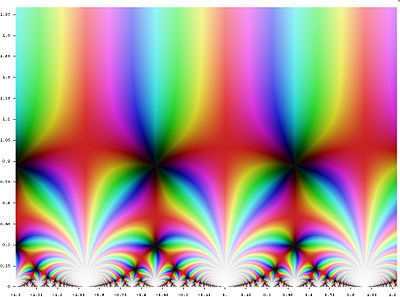
\includegraphics[width=\textwidth]{400px-KleinInvariantJ.jpg}
    {\tiny Image source: Jan Homann (wikipedia)}
  \end{center}
\end{minipage}
  \begin{minipage}{0.58\linewidth}
      Klein's $j$-function is
  holomorphic on $\IH$ and meromorphic at infinity.

  It satisfies  $j(\tau)=j(\tau+1)$, so $j(\tau)$ depends only
  on $q=e^{2\pi i \tau}$. 
  \begin{equation*}
    j(q) = \frac 1q + 744 + 196884q +\cdots. 
  \end{equation*}
  \end{minipage}
\end{frame}

\begin{frame}
  \begin{definition}    
    A \alert{special point} of $Y(1)$ is the $j$-invariant of an elliptic curve
    with complex multiplication; equivalently a member of 
    $\{j(\tau) : \tau\in\IH \text{ and }[\IQ(\tau):\IQ]=2\}$.

    For $m\ge 1$ we define
    $$
    Y(1)^m_{\mathrm{special}} = \{(z_1,\ldots,z_m)\in\IC^m : z_j \text{ is
      special in $Y(1)$ for all $j$}\}.
    $$
  \end{definition}
\end{frame}

\begin{frame}
  Basic idea of the Andr\'e--Oort Conjecture: A curve in $Y(1)^2$
  contains only finitely many special points except if there is a good
  reason why not. 

  \begin{example}
    \begin{enumerate}
    \item[(i)] The diagonal  $\{(z,z) : z\in\IC\}$ contains infinitely
      many special points of $Y(1)^2$. 
    \item [(ii)]  Let $z$ be a special point of $Y(1)$.  Then the curves
      $\{z\}\times Y(1)$ and $Y(1)\times \{z\}$ contain infinitely many
      special points of $Y(1)^2$. 
    \end{enumerate}
  \end{example}

  So we should declare the diagonal as well as horizonal and vertical
  lines whose fixed coordinate is  special, as special curves.

  But there are more special curves!
\end{frame}

\begin{frame}
  \begin{definition}
    An \alert{isogeny} $f\colon E_1\rightarrow E_2$ of elliptic curves, both
    defined over $\IC$, is a non-constant morphism
    of algebraic varieties with $f(0)=0$. 
  \end{definition}
  
  If $E_i$ is represented by $\IC/(\IZ+\tau_i\IZ)$,
  then $f$ is represented by $\alpha\in\IC^\times$ with 
   $\alpha(\IZ+\tau_1\IZ)\subset \IZ+\tau_2\IZ$. An isogeny induces a \alert{group
   homomorphism} $E_1(\IC)\rightarrow E_2(\IC)$

  We call $f$ a \alert{cyclic isogeny}, if $\mathrm{ker}(f)$ is a cycle
  group.

  \begin{lemma}
    For $N\in\IN$, 
    \begin{equation*}
      \left\{ (j(\tau_1),j(\tau_2)) : \text{ 
          $\exists \IC/(\IZ+\tau_1\IZ)\rightarrow \IC/(\IZ+\tau_2\IZ)$ cyclic of degree $N$}\right\}
    \end{equation*}
    is the
    the zero set of a geometrically irreducible $\Phi_N\in\IZ[X,Y]$.
  \end{lemma}

  The zero set of $\Phi_N$ contains infinitely many special points. 
\end{frame}

\begin{frame}
  \begin{example}
    \begin{enumerate}
    \item [(i)]    For $N=1$ we recover the diagonal, 
      $\Phi_1 = X-Y$.
    \item[(ii)] For $N=2$ we have   
      \begin{alignat*}1
        \Phi_2 = 
        \,\,&X^3 - X^2Y^2 + 1488X^2Y - 162000X^2 + 1488XY^2 \\
        &+ 40773375XY +
        8748000000X +Y^3 - 162000Y^2 \\
        &+ 8748000000Y -157464000000000.    
      \end{alignat*}
    \end{enumerate}
  \end{example}
  \vspace{-0.5cm}
  \begin{equation*}
    \deg_X \Phi_N = N\prod_{p\mid N}\left(1+\frac 1p\right). 
  \end{equation*}
 
  Cohen: coefficients of $\Phi_N$ grow superexponentially in $N$.
  
  \begin{definition}
    The $\Phi_N$ are called \alert{modular transformation polynomials}.
  \end{definition}
\end{frame}

\begin{frame}{Andr\'e--Oort for $Y(1)^2$}
  \begin{definition}
    An algebraic curve  $C\subset Y(1)^2$ is called a \alert{special curve} of
    $Y(1)^2$ 
    \begin{enumerate}
    \item [(i)] if $C = \{z\}\times Y(1)$ for a special point $z$, or
    \item [(ii)] if $C =  Y(1)\times \{z\}$ for a special point $z$, or
    \item[(iii)] if $C=Z(\Phi_N)$ for some $N\in\IN$. 
    \end{enumerate}
  \end{definition}

  \begin{theorem}[Andr\'e--Oort for $Y(1)^2$]
    Let $C\subset Y(1)^2$ be an irreducible curve. Then
    \begin{equation*}
      C \cap Y(1)^2_{\mathrm{special}}\text{ is
        infinite}\quad\Longleftrightarrow\quad \text{$C$ is a special
        curve of $Y(1)^2$}. 
    \end{equation*}  
  \end{theorem}

  \vspace{-0.25cm}
  Many proofs: Andr\'e, Edixhoven under GRH, Pila for subvarieties of
  $Y(1)^m$, effective versions by Bilu--Masser--Zannier and K\"uhne.
  Generalizations by: Klingler, Tsimerman, Ullmo, Yafaev, \ldots
\end{frame}

\begin{frame}{Galois Theory of Special Points}  
  \begin{theorem}
    Let $z\in Y(1)_{\mathrm{special}}$ with $z=j(\tau)$ where
    $\tau\in \IH$. Let $F=\IQ(\tau)$.
    \begin{enumerate}
    \item [(i)] Then $z$ is an algebraic integer.
    \item[(ii)]  $F$ is
      imaginary quadratic and   $\mathrm{End}(E)$ is an order
      in $F$.
    \item[(iii)] The extension $F(z)/F$ is Galois with abelian Galois
      group.
    \item[(iv)] If $\mathrm{End}(E)$ is the ring of integers of $F$, then
      the class group $H_F$ of $F$ is isomorphic to
      $\mathrm{Gal}(F(z)/F)$.
      Moreover, $F(z)$ is the Hilbert Class Field of $F$. 
    \end{enumerate}
  \end{theorem}
  \begin{example}
    \begin{enumerate}
    \item [(i)] $j$-invariant $1728$ corresponds to $y^2 = x^3+x$, here
      $\mathrm{End}(E) = \IZ[i]$ has class number $1$,
      $F=\IQ(i)$,
      $F(z)=F$
    \end{enumerate}
  \end{example}
\end{frame}

\begin{frame}
  \begin{example}[continued]
    \begin{enumerate}
    \item[(ii)] $j$-invariant $282880 \sqrt{5}-632000$ corresponds to
      $\IC/(\IZ+\sqrt{-5}\IZ)$, here $\mathrm{End}(E)=\IZ[\sqrt{-5}]$
      has class number $2$, $F=\IQ(\sqrt{-5})$, and $F =
      \IQ(i,\sqrt{5})$. 
    \end{enumerate}
  \end{example}

  Edixhoven's proof is related to Serre and Tate's proof above.
  \begin{theorem}[Edixhoven: Andr\'e--Oort for $Y(1)^2$]
    Suppose the Generalized Riemann Hypothesis (GRH) holds true. 
    Let $C\subset Y(1)^2$ be an irreducible curve. If
    \begin{equation*}
      C \cap Y(1)^2_{\mathrm{special}}\text{ is
        infinite, then}
    \end{equation*}
    \vspace{-0.75cm}
    \begin{enumerate}
    \item [(i)] $C$ is a horizontal or vertical line whose fixed coordinate
      is  special, or
    \item[(ii)] $C=Z(\Phi_N)$ for some $N\in\IN$. 
    \end{enumerate}
  \end{theorem}
\end{frame}

\begin{frame}{Preliminary Remarks}
  \textbf{Reduction step: We may assume $C=Z(P)$ with $P\in\IQbar[X,Y]$.} This
  is identical as in the Ihara--Serre-Tate. Indeed, special points of
  $Y(1)^2$ are algebraic.

  So there are finitely $(z_1,z_2) \in Y(1)^2_{\mathrm{special}}$ with
  $P(z_1,z_2)=0$.

  Write $z_1=j(\tau_1)$ and $z_2=j(\tau_2)$ with $\tau_{1,2}\in\IH$
  and $E_{1,2} = \IC/(\IZ+\tau_{1,2}\IZ)$.
  
  \textbf{We make two simplifying assumptions:}
  

  \begin{enumerate}
  \item [(i)] Assume $\mathrm{End}(E_{1,2})$ are \alert{maximal
      orders}, so rings of integers in their field of fractions.

  \item[(ii)] We assume $F = \IQ(\mathrm{End}(E_1)) =
    \IQ(\mathrm{End}(E_2))$, both $CM$-fields are equal. This implies
    that $E_1$ and $E_2$ are isogenous. 
  \end{enumerate}
  Let $\Delta$ be the
  discriminant of $F$. 
\end{frame}

\begin{frame}{The Galois Orbit}
  \begin{lemma}[Large Galois Orbit]
    We have
      $\# \mathrm{Gal}(\IQ(z_1,z_2)/\IQ) \gg_\epsilon
      |\Delta|^{1/4}$.
  \end{lemma}
  \begin{proof}
    The left-hand side is at least the order of the class group $H_F$
    of the imaginary quadratic number field $F$. The Landau--Siegel Theorem
    implies $\# H_F \gg_\epsilon |\Delta|^{1/2-\epsilon}$ for any $\epsilon>0$. 
    The lemma follows with the choice $\epsilon =1/4$. 
  \end{proof}

\end{frame}
\begin{frame}{Galois Homothety}
  The analog of the Galois Homothety Lemma is more subtle because
  there is no natural group law.
  But for all $N\in\IN$
  we have \alert{Hecke correspondences}:
  \begin{equation*}
    \begin{tikzcd}[ampersand replacement=\&,column sep=small, row sep=small] 
      \& \{(z,w,z',w') : \Phi_N(z,z')=\Phi_N(w,w')=0\} \arrow{ddl}[swap]{} \arrow{ddr}{} \&\\
      \&  \&\\[-2ex]
      Y(1)^2  \& \& Y(1)^2 \\
    \end{tikzcd}
  \end{equation*}
  
  \begin{definition}
    \begin{alignat*}1
      T_N(C) := \{(z,w) \in\IC^2 : &\text{there exists $(z',w')\in C$}\\
      &\text{with $\Phi_N(z,z')=\Phi_N(w,w')=0$}\}
    \end{alignat*}
    is a possibly reducible algebraic curve in $Y(1)^2$. 
  \end{definition}
\end{frame}

\begin{frame}
  \begin{lemma}[Galois Homothety Lemma]
    Suppose the \alert{GRH}.
    Say $(z_1,z_2)\in Y(1)^2$ is as above.
    There exists a prime number $\ell=O((\log
    |\Delta|)^3)$ and $\sigma\in \mathrm{Gal}(\IQbar/\IQ)$
    with $\Phi_\ell(z_1,\sigma(z_1))=\Phi_\ell(z_2,\sigma(z_2))=0$. 
  \end{lemma}
  \begin{proof}
    \vspace{4cm}
  \end{proof}
\end{frame}

\begin{frame}{Putting Things Together}
  
  The \alert{Galois Homothety Lemma} implies $P(z_1,z_2)=0$, $P(\sigma(z_1),\sigma(z_1))=0,$
  and $\Phi_\ell(z,\sigma(z))=\Phi_\ell(w,\sigma(w))=0$ for some
  $\sigma\in\mathrm{Gal}(\IQbar/\IQ)$ and some prime
  $\ell \ll (\log|\Delta|)^3$. 
  \begin{equation*}
    \Longrightarrow (z_1,z_2) \in C \cap T_\ell(C).
  \end{equation*}
  The
  intersection $C\cap T_\ell(C)$ is {fixed} by the action
  $\mathrm{Gal}(\IQbar/\IQ)$. The \alert{Large Galois Orbit Lemma} implies
  \begin{equation}
      |\Delta|^{1/4} \ll \# C\cap
    T_\ell(C).
  \end{equation}
  Basic degree estimates  yield $\deg T_\ell(C) \ll \ell^2 \ll (\log|\Delta|)^6$.
  \begin{equation*}
    \text{\alert{B\'ezout}} \Longrightarrow \# C\cap T_\ell(C) \ll \deg
    T_{\ell}(C)\ll (\log|\Delta|)^6.
  \end{equation*}
  \begin{equation*}
    \Longrightarrow
    |\Delta|^{1/4} \ll (\log |\Delta|)^6 \Longrightarrow |\Delta|\ll 1
  \end{equation*}

  But bounding $|\Delta|$ means $(z_1,z_2)$ is in a finite set. 
\end{frame}

\begin{frame}{Wait!}
  This argument must contain a \alert{gap}! Not all curves in $Y(1)^2$
  contain only finitely many special points, \textit{e.g.}, special
  curves.  Where did it go wrong?

  When applying B\'ezout's Theorem we assumed that $C\cap T_\ell(C)$
  was finite.

  What happens when $C\subset T_\ell(C)$? This situation corresponds
  to $C\subset [\ell]^{-1}(C)$ in the proof of the
  Ihara--Serre--Tate Theorem. 

  \begin{theorem}[Edixhoven]
    Suppose $\ell$ is a prime number, sufficiently large in terms of
    $C$ with $C\subset [\ell]^{-1}(C)$. Then $C$ is a special curve of
    $Y(1)^2$. 
  \end{theorem}

  We will see a different proof of this result towards the end of this
  week.   
\end{frame}

\begin{frame}{Conclusion}

  \begin{itemize}
  \item The set of special points of $\IG_{\mathrm{m}}^2$ are the
    torsion points of $(\IC^\times)^2$, \textit{i.e.},  the image
    of $\IQ^2$ under $$(q_1,q_2)\mapsto (\exp(2\pi i
    q_1),\exp(2\pi iq_2)).$$ 
    Ihara--Serre--Tate Theorem: The only algebraic curves in $\IG_{\mathrm{m}}^2$ that
    contain infinitely many special points are translates of algebraic
    subgroups by torsion points.

  \item Special points of $Y(1)^2$  correspond
    to products of elliptic curves with complex multiplication. The
    set of special points also equals 
    the image of all imaginary quadratic elements in
    $\IH^2$ under
    $$ (\tau_1,\tau_2) \mapsto (j(\tau_1),j(\tau_2)).$$
    Andr\'e--Edixhoven: The only algebraic curves in $Y(1)^2$ that
    contain infinitely many special points are horizonal, vertical, or
    come from the modular transformation polynomials $\Phi_N$. 
  \end{itemize}
\end{frame}

\begin{frame}
  \begin{center}
    Thanks for your attention.

    See you tomorrow when we begin o-minimal geometry.
  \end{center}
\end{frame}
\end{document}
